\chapter{Variables aléatoires}

\section{Variable aléatoire et loi de probabilité}

\subsection{Variable aléatoire}

\begin{ex}
	Soit l'expérience aléatoire : \og On lance un dé à six faces et on regarde le résultat \fg{}.

	L'ensemble de toutes les issues possibles s'appelle l'\textbf{univers des possibles} : $\Omega = \brac{\epsdice{1}\,;\,\epsdice{2}\,;\,\epsdice{3}\,;\,\epsdice{4}\,;\,\epsdice{5}\,;\,\epsdice{6}}$

	\begin{center}
		\begin{tikzpicture}[>=Stealth, scale=0.8]
			\draw[gray!60, line width=2pt, rounded corners=8pt] (-0.2, 0.2) rectangle (2.6, 5.0);
			\node[above, font=\large] at (1.2, 5.0) {$\Omega$};
			\draw[gray!60, line width=2pt, rounded corners=8pt] (4.0, 0.8) rectangle (5.9, 4.4);
			\node[above, font=\large] at (4.95, 4.4) {$X(\Omega)$};
			\draw[rounded corners=2pt, fill=white] (1.2, 4.1) rectangle (1.8, 4.7);
			\fill (1.5, 4.4) circle (2pt);
			\draw[rounded corners=2pt, fill=white] (0.2, 3.3) rectangle (0.8, 3.9);
			\fill (0.35, 3.75) circle (2pt);
			\fill (0.65, 3.45) circle (2pt);
			\draw[rounded corners=2pt, fill=white] (1.2, 2.7) rectangle (1.8, 3.3);
			\fill (1.35, 3.15) circle (2pt);
			\fill (1.5, 3.0) circle (2pt);
			\fill (1.65, 2.85) circle (2pt);
			\draw[rounded corners=2pt, fill=white] (0.2, 1.9) rectangle (0.8, 2.5);
			\fill (0.35, 2.35) circle (2pt);
			\fill (0.65, 2.35) circle (2pt);
			\fill (0.35, 2.05) circle (2pt);
			\fill (0.65, 2.05) circle (2pt);
			\draw[rounded corners=2pt, fill=white] (1.2, 1.1) rectangle (1.8, 1.7);
			\fill (1.35, 1.55) circle (2pt);
			\fill (1.65, 1.55) circle (2pt);
			\fill (1.5, 1.4) circle (2pt);
			\fill (1.35, 1.25) circle (2pt);
			\fill (1.65, 1.25) circle (2pt);
			\draw[rounded corners=2pt, fill=white] (0.2, 0.4) rectangle (0.8, 1.0);
			\fill (0.35, 0.85) circle (2pt);
			\fill (0.65, 0.85) circle (2pt);
			\fill (0.35, 0.7) circle (2pt);
			\fill (0.65, 0.7) circle (2pt);
			\fill (0.35, 0.55) circle (2pt);
			\fill (0.65, 0.55) circle (2pt);
			\node (m1) at (4.95, 3.6) {$-1$};
			\node (p2) at (4.95, 1.6) {$2$};
			\draw[->, thick, shorten >= -3pt] (1.9, 4.4) to[out=10, in=145] (m1);
			\draw[->, thick, shorten >= -3pt] (0.9, 3.6) to[out=10, in=175] (m1);
			\draw[->, thick, shorten >= -3pt] (1.9, 3.0) to[out=15, in=195] (m1);
			\draw[->, thick, shorten >= -3pt] (0.9, 2.2) to[out=20, in=215] (m1);
			\draw[->, thick, shorten >= -3pt] (1.9, 1.4) to[out=15, in=165] (p2);
			\draw[->, thick, shorten >= -3pt] (0.9, 0.7) to[out=-10, in=205] (p2);
		\end{tikzpicture}
	\end{center}

	On considère le jeu suivant :
	\begin{itemize}
		\item Si le résultat est \epsdice{5} ou \epsdice{6}, on gagne $2\eur{}$.
		\item Sinon, on perd $1\eur{}$.
	\end{itemize}

	On peut définir ainsi une variable aléatoire $X$ qui donne \textbf{le gain} du joueur. $X$ peut prendre les valeurs $2$ ou $-1$.
	\begin{itemize}
		\item Pour les issues \epsdice{5} et \epsdice{6}, on a $X = 2$.
		\item Pour les issues \epsdice{1}, \epsdice{2}, \epsdice{3} et \epsdice{4}, on a $X = -1$.
	\end{itemize}
\end{ex}

\begin{defin}
	Une \textbf{variable aléatoire} $X$ associe un nombre réel à chaque issue de l'univers d'une expérience aléatoire :
	\[
		\begin{array}{rcl}
			\Omega & \longrightarrow & \R     \\
			e_i    & \longmapsto     & X(e_i)
		\end{array}
	\]
\end{defin}

\begin{ex}
	\nline
	\begin{enumerate}
		\item \textbf{Nombre de succès :} Soit $X$ la variable aléatoire représentant le nombre de piles obtenus après $10$ lancers d'une pièce équilibrée.
		      \[
			      X(\Omega) = \brac{0\,;\,1\,;\,2\,;\,\dots\,;\,10}
		      \]
		\item \textbf{Concentration sanguine :} Soit $X$ la variable aléatoire mesurant le taux de glycémie à jeun (en g/L) arrondi au dixième lors d'un bilan médical d'un patient pris au hasard.
		      \[
			      X(\Omega) = \brac{0{,}7\,;\,0{,}8\,;\,0{,}9\,;\,1{,}0\,;\,1{,}1\,;\,1{,}2}
		      \]
		\item \textbf{Nombre de frères et sœurs :} Soit $X$ la variable aléatoire représentant le nombre de frères et sœurs d'un élève choisi au hasard dans un lycée.
		      \[
			      X(\Omega) = \brac{0\,;\,1\,;\,2\,;\,3\,;\,\dots}
		      \]
	\end{enumerate}
\end{ex}

\begin{methode}[Calculer une probabilité à l'aide d'une variable aléatoire]
	On tire une carte au hasard dans un jeu de $32$ cartes.

	\begin{itemize}
		\item Si cette carte est un c\oe ur ($\heartsuit$), on gagne $5\eur{}$.
		\item Si cette carte est un pique ($\spadesuit$), on gagne $2\eur{}$.
		\item Dans les autres cas, on perd $1\eur{}$.
	\end{itemize}

	Soit $X$ la variable aléatoire égale au gain du jeu.

	Calculons $\p{X=5}$, $\p{X=-1}$ et $\p{X \le 2}$.

	\begin{correction}
		\nline
		\begin{itemize}
			\item $\p{X=5}$ est la probabilité de gagner $5\eur{}$.

			      On gagne $5\eur{}$ lorsqu'on tire un c\oe ur ($\heartsuit$).
			      \[
				      \p{X=5} = \dfrac{8}{32} = \dfrac{1}{4}
			      \]

			\item $\p{X=-1}$ est la probabilité de perdre $1\eur{}$.

			      On perd $1\eur{}$ lorsqu'on ne tire ni un c\oe ur, ni un pique.
			      \[
				      \p{X=-1} = \dfrac{16}{32} = \dfrac{1}{2}
			      \]

			\item $\p{X \le 2}$ est la probabilité de gagner au plus $2\eur{}$.
			      \[
				      \p{X \le 2} = \p{X=2} + \p{X=-1} = \dfrac{1}{4} + \dfrac{1}{2} = \dfrac{3}{4}
			      \]
		\end{itemize}
	\end{correction}
\end{methode}

\subsection{Loi de probabilité}

\begin{defin}
	Soit une variable aléatoire $X$ prenant les valeurs $x_{1}, x_{2}, \dots, x_{n}$.

	La \textbf{loi de probabilité} de $X$ associe à chaque valeur $x_i$ la probabilité $\p{X=x_{i}}$.

	\begin{center}
		\rnc{\arraystretch}{1.4}
		\begin{tabular}{|c|c|c|c|c|} \hline
			\ccg $x_i$       & $x_1$ & $x_2$ & $\dots$ & $x_n$ \\ \hline
			\ccg $\p{X=x_i}$ & $p_1$ & $p_2$ & $\dots$ & $p_n$ \\ \hline
		\end{tabular}
	\end{center}
\end{defin}

\begin{remarque}
	Les $x_{i}$ sont l'ensemble des valeurs distinctes prises par la variable aléatoire $X$.
\end{remarque}

\begin{ex}
	On observe la présence d'un élève au cours d'une semaine de $5$ jours de classe.

	Soit $X$ la variable aléatoire qui associe à cette semaine le nombre de jours où l'élève est en retard.

	Les valeurs possibles pour $X$ sont $0$, $1$, $2$, $3$, $4$ et $5$.

	La loi de probabilité de $X$ donne la probabilité de chaque nombre de retards :

	\begin{center}
		\rnc{\arraystretch}{1.5}
		\begin{tabular}{|c|c|c|c|c|c|c|} \hline
			\ccg $x_i$       & $0$      & $1$      & $2$      & $3$      & $4$      & $5$      \\ \hline
			\ccg $\p{X=x_i}$ & $0{,}60$ & $0{,}25$ & $0{,}10$ & $0{,}03$ & $0{,}01$ & $0{,}01$ \\ \hline
		\end{tabular}
	\end{center}

	À partir de cette loi, on peut calculer la probabilité de différents événements :
	\begin{itemize}
		\item La probabilité que cet élève soit en retard exactement $2$ jours dans la semaine :
		      \[
			      \p{X=2} = 0{,}10 \quad (\text{soit } 10\,\%)
		      \]
		\item La probabilité d'avoir au moins $3$ retards dans la semaine ($X \ge 3$) :
		      \[
			      \begin{array}{rccccccl}
				      \p{X \ge 3} & = & \p{X=3} & + & \p{X=4} & + & \p{X=5} &          \\
				                  & = & 0{,}03  & + & 0{,}01  & + & 0{,}01  & = 0{,}05
			      \end{array}
		      \]
		      \textbf{Interprétation :}

			  Il y a $5\,\%$ de chances que l'élève accumule $3$ retards ou plus au cours de la semaine.
	\end{itemize}
\end{ex}

\begin{methode}[Déterminer la loi de probabilité d'une variable aléatoire]
	On lance simultanément deux dés équilibrés à $6$ faces et on note les valeurs obtenues.

	Soit $X$ la variable aléatoire égale à \textbf{la plus grande des deux valeurs}.

	Établissons la loi de probabilité de $X$.

	\begin{correction}
		La variable aléatoire $X$ peut prendre les valeurs $1$, $2$, $3$, $4$, $5$ et $6$.

		Par exemple, si on obtient la combinaison $\pa{\epsdice{2}\,;\,\epsdice{5}}$, la plus grande valeur est $5$ et on a $X=5$.

		On peut modéliser l'ensemble des éventualités à l'aide d'un tableau :
		\[
			\rnc{\arraystretch}{1.3}
			\begin{array}{|c|c|c|c|c|c|c|}\hline
				X           & \epsdice{1}    & \epsdice{2}    & \epsdice{3}    & \epsdice{4}    & \epsdice{5}    & \epsdice{6} \\ \hline
				\epsdice{1} & \cc{gray!60} 1 & \cc{gray!48} 2 & \cc{gray!36} 3 & \cc{gray!24} 4 & \cc{gray!12} 5 & 6           \\ \hline
				\epsdice{2} & \cc{gray!48} 2 & \cc{gray!48} 2 & \cc{gray!36} 3 & \cc{gray!24} 4 & \cc{gray!12} 5 & 6           \\ \hline
				\epsdice{3} & \cc{gray!36} 3 & \cc{gray!36} 3 & \cc{gray!36} 3 & \cc{gray!24} 4 & \cc{gray!12} 5 & 6           \\ \hline
				\epsdice{4} & \cc{gray!24} 4 & \cc{gray!24} 4 & \cc{gray!24} 4 & \cc{gray!24} 4 & \cc{gray!12} 5 & 6           \\ \hline
				\epsdice{5} & \cc{gray!12} 5 & \cc{gray!12} 5 & \cc{gray!12} 5 & \cc{gray!12} 5 & \cc{gray!12} 5 & 6           \\ \hline
				\epsdice{6} & 6              & 6              & 6              & 6              & 6              & 6           \\ \hline
			\end{array}
		\]

		L'univers comporte $36$ issues équiprobables.

		En comptant les apparitions de chaque valeur, on obtient :
		\begin{multicols}{3}
			\begin{itemize}
				\item $\p{X=1} = \dfrac{1}{36}$
				\item $\p{X=2} = \dfrac{3}{36}$
				\item $\p{X=3} = \dfrac{5}{36}$
				\item $\p{X=4} = \dfrac{7}{36}$
				\item $\p{X=5} = \dfrac{9}{36}$
				\item $\p{X=6} = \dfrac{11}{36}$
			\end{itemize}
		\end{multicols}

		On résume ces résultats dans le tableau de la loi de probabilité de $X$ :

		\begin{center}
			\rnc{\arraystretch}{1.5}
			\begin{tabular}{|c|c|c|c|c|c|c|} \hline
				\ccg $x_i$                             & $1$             & $2$             & $3$             & $4$             & $5$             & $6$              \\ \hline
				\rule[-4mm]{0mm}{11mm}\ccg $\p{X=x_i}$ & $\dfrac{1}{36}$ & $\dfrac{3}{36}$ & $\dfrac{5}{36}$ & $\dfrac{7}{36}$ & $\dfrac{9}{36}$ & $\dfrac{11}{36}$ \\ \hline
			\end{tabular}
		\end{center}
	\end{correction}

	On peut vérifier que la somme de toutes les probabilités est bien égale à $1$ :
	\[
		\dfrac{1}{36} + \dfrac{3}{36} + \dfrac{5}{36} + \dfrac{7}{36} + \dfrac{9}{36} + \dfrac{11}{36} = \dfrac{36}{36} = 1
	\]

	À partir de cette loi, on peut calculer la probabilité d'événements plus complexes :

	\begin{itemize}
		\item La probabilité que la plus grande valeur soit supérieure ou égale à $5$ ($X \ge 5$) :
		      \[
			      \begin{array}{rccccl}
				      \p{X \ge 5} & = & \p{X=5}       & + & \p{X=6}        &                                                \\
				                  & = & \dfrac{9}{36} & + & \dfrac{11}{36} & = \dfrac{20}{36} = \dfrac{5}{9} \approx 0{,}56
			      \end{array}
		      \]
		      \textbf{Interprétation :} 

			  Il y a environ $56\,\%$ de chances que le plus grand nombre obtenu sur les deux dés soit au moins égal à $5$.

		\item La probabilité que la plus grande valeur soit strictement inférieure à $3$ :
		      \[
			      \begin{array}{rccccl}
				      \p{X < 3} & = & \p{X=1}       & + & \p{X=2}       &                                               \\
				                & = & \dfrac{1}{36} & + & \dfrac{3}{36} & = \dfrac{4}{36} = \dfrac{1}{9} \approx 0{,}11
			      \end{array}
		      \]
		      \textbf{Interprétation :}

			  La probabilité d'obtenir un maximum strictement inférieur à $3$ est de $1$ chance sur $9$ (soit environ $11\,\%$).
	\end{itemize}
\end{methode}

\section{Espérance mathématique}

\subsection{Définition et interprétation}

\begin{defin}
	Soit une variable aléatoire $X$ dont la loi de probabilité est donnée par le tableau suivant :

	\begin{center}
		\rnc{\arraystretch}{1.4}
		\begin{tabular}{|c|c|c|c|c|} \hline
			\ccg $x_i$       & $x_1$ & $x_2$ & $\dots$ & $x_n$ \\ \hline
			\ccg $\p{X=x_i}$ & $p_1$ & $p_2$ & $\dots$ & $p_n$ \\ \hline
		\end{tabular}
	\end{center}

	L'\textbf{espérance mathématique} de la variable aléatoire $X$, notée $E(X)$, est le nombre réel défini par :
	\[
		E(X) = p_{1}x_{1} + p_{2}x_{2} + \dots + p_{n}x_{n} = \sum_{i=1}^{n} p_i x_i
	\]
\end{defin}

\begin{remarque}
	L'espérance mathématique $E(X)$ correspond à la \textbf{moyenne} des valeurs $x_i$ prises par la variable aléatoire, pondérées par leurs probabilités $p_i$.
\end{remarque}

\begin{ex}
	Reprenons l'exemple du lancer de deux dés où $X$ représente la plus grande des deux valeurs :

	\begin{center}
		\rnc{\arraystretch}{1.5}
		\begin{tabular}{|c|c|c|c|c|c|c|} \hline
			\ccg $x_i$                             & $1$             & $2$             & $3$             & $4$             & $5$             & $6$              \\ \hline
			\rule[-4mm]{0mm}{11mm}\ccg $\p{X=x_i}$ & $\dfrac{1}{36}$ & $\dfrac{3}{36}$ & $\dfrac{5}{36}$ & $\dfrac{7}{36}$ & $\dfrac{9}{36}$ & $\dfrac{11}{36}$ \\ \hline
		\end{tabular}
	\end{center}

	\textbf{Calcul de l'espérance :}
	\[
		\def\arraystretch{2}
		\begin{array}{rccccccccccccl}
			E(X) & = & 1 \times \dfrac{1}{36} & + & 2 \times \dfrac{3}{36} & + & 3 \times \dfrac{5}{36} & + & 4 \times \dfrac{7}{36} & + & 5 \times \dfrac{9}{36} & + & 6 \times \dfrac{11}{36} &                                   \\
			     & = & \dfrac{1}{36}          & + & \dfrac{6}{36}          & + & \dfrac{15}{36}         & + & \dfrac{28}{36}         & + & \dfrac{45}{36}         & + & \dfrac{66}{36}          & = \dfrac{161}{36}  \approx 4{,}47
		\end{array}
	\]

	\textbf{Interprétation :}

	En répétant cette expérience un très grand nombre de fois, la valeur moyenne de la plus grande des deux faces obtenues est d'environ $4{,}47$.
\end{ex}

\newpage

\begin{methode}[Calculer l'espérance d'une variable aléatoire]
	\nline
	\begin{wrapstuff}[r]
		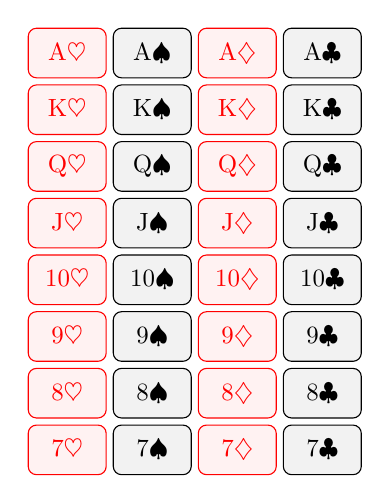
\begin{tikzpicture}[scale=0.9, transform shape]
			\tikzset{
				card/.style={draw, rounded corners=3pt, minimum width=1.1cm, minimum height=0.7cm, align=center},
				cardr/.style={card, draw=red, text=red, fill=red!5!white},
				cordb/.style={card, draw=black, text=black, fill=black!5!white}
			}
			\node[cardr] (c1) at (0, 0) {A$\heartsuit$}; \node[cardr] (c2) at (0, -0.8) {K$\heartsuit$}; \node[cardr] (c3) at (0, -1.6) {Q$\heartsuit$}; \node[cardr] (c4) at (0, -2.4) {J$\heartsuit$};
			\node[cardr] (c5) at (0, -3.2) {10$\heartsuit$}; \node[cardr] (c6) at (0, -4.0) {9$\heartsuit$}; \node[cardr] (c7) at (0, -4.8) {8$\heartsuit$}; \node[cardr] (c8) at (0, -5.6) {7$\heartsuit$};
			\node[cordb] (s1) at (1.2, 0) {A$\spadesuit$}; \node[cordb] (s2) at (1.2, -0.8) {K$\spadesuit$}; \node[cordb] (s3) at (1.2, -1.6) {Q$\spadesuit$}; \node[cordb] (s4) at (1.2, -2.4) {J$\spadesuit$};
			\node[cordb] (s5) at (1.2, -3.2) {10$\spadesuit$}; \node[cordb] (s6) at (1.2, -4.0) {9$\spadesuit$}; \node[cordb] (s7) at (1.2, -4.8) {8$\spadesuit$}; \node[cordb] (s8) at (1.2, -5.6) {7$\spadesuit$};
			\node[cardr] (d1) at (2.4, 0) {A$\diamondsuit$}; \node[cardr] (d2) at (2.4, -0.8) {K$\diamondsuit$}; \node[cardr] (d3) at (2.4, -1.6) {Q$\diamondsuit$}; \node[cardr] (d4) at (2.4, -2.4) {J$\diamondsuit$};
			\node[cardr] (d5) at (2.4, -3.2) {10$\diamondsuit$}; \node[cardr] (d6) at (2.4, -4.0) {9$\diamondsuit$}; \node[cardr] (d7) at (2.4, -4.8) {8$\diamondsuit$}; \node[cardr] (d8) at (2.4, -5.6) {7$\diamondsuit$};
			\node[cordb] (t1) at (3.6, 0) {A$\clubsuit$}; \node[cordb] (t2) at (3.6, -0.8) {K$\clubsuit$}; \node[cordb] (t3) at (3.6, -1.6) {Q$\clubsuit$}; \node[cordb] (t4) at (3.6, -2.4) {J$\clubsuit$};
			\node[cordb] (t5) at (3.6, -3.2) {10$\clubsuit$}; \node[cordb] (t6) at (3.6, -4.0) {9$\clubsuit$}; \node[cordb] (t7) at (3.6, -4.8) {8$\clubsuit$}; \node[cordb] (t8) at (3.6, -5.6) {7$\clubsuit$};
		\end{tikzpicture}
	\end{wrapstuff}
	On tire une carte dans un jeu de $32$ cartes.

	\begin{itemize}
		\item Si on tire un c\oe ur ($\heartsuit$), on gagne $2\eur{}$.
		\item Si on tire un Roi ($K$), on gagne $5\eur{}$.
		\item Si on tire une autre carte, on perd $1\eur{}$.
	\end{itemize}

	Soit $X$ la variable aléatoire donnant le gain algébrique du joueur.

	Calculons l'espérance de $X$.

	\rule{0mm}{25mm}

	\begin{correction}
		$X$ peut prendre les valeurs $-1\eur{}$, $2\eur{}$, $5\eur{}$ ainsi que $7\eur{}$.

		En effet, si la carte tirée est le Roi de c\oe ur, on cumule le gain du c\oe ur ($2\eur{}$) et celui du Roi ($5\eur{}$), soit $7\eur{}$.
		\[
			X(\Omega) = \brac{-1\,;\,2\,;\,5\,;\,7}
		\]

		Déterminons la probabilité de chaque valeur :
		\begin{itemize}
			\item Roi de c\oe ur : $X = 7$ avec $\p{X=7} = \dfrac{1}{32}$.
			\item Autre Roi (Pique, Trèfle, Carreau) : $X = 5$ avec $\p{X=5} = \dfrac{3}{32}$.
			\item Autre c\oe ur (hors Roi) : $X = 2$ avec $\p{X=2} = \dfrac{7}{32}$.
			\item Carte ni c\oe ur ni Roi : $X = -1$ avec $\p{X=-1} = \dfrac{21}{32}$.
		\end{itemize}

		\textbf{Loi de probabilité de $X$ :}

		\begin{center}
			\rnc{\arraystretch}{1.5}
			\begin{tabular}{|c|c|c|c|c|} \hline
				\ccg $x_i$                             & $-1$             & $2$             & $5$             & $7$             \\ \hline
				\rule[-4mm]{0mm}{11mm}\ccg $\p{X=x_i}$ & $\dfrac{21}{32}$ & $\dfrac{7}{32}$ & $\dfrac{3}{32}$ & $\dfrac{1}{32}$ \\ \hline
			\end{tabular}
		\end{center}

		\textbf{Calcul de l'espérance :}
		\[
			\def\arraystretch{2}
			\begin{array}{rccccccccl}
				E(X) & = & \pa{-1} \times \dfrac{21}{32} & + & 2 \times \dfrac{7}{32} & + & 5 \times \dfrac{3}{32} & + & 7 \times \dfrac{1}{32} &                                 \\
				     & = & \dfrac{-21}{32}               & + & \dfrac{14}{32}         & + & \dfrac{15}{32}         & + & \dfrac{7}{32}          & = \dfrac{15}{32} \approx 0{,}47
			\end{array}
		\]

		\textbf{Interprétation :}

		Si l'on répète l'expérience un grand nombre de fois, le joueur peut espérer gagner en moyenne environ $0{,}47\eur{}$ par partie.

		Pour rendre le jeu équitable ou avantageux pour l'organisateur, ce dernier devrait demander une participation d'au moins $0{,}47\eur{}$ (par exemple $0{,}50\eur{}$) par partie.
	\end{correction}
\end{methode}
